% ================================================================
%  jabri_5.tex — Zeros of the Al-Jabri Field
%  Author: Eng. Abdulla M. N. Al-Jabri — Sana'a, Yemen
%  October 2026
% ================================================================

\documentclass[11pt,a4paper]{article}
\usepackage[utf8]{inputenc}
\usepackage{amsmath,amssymb,amsthm}
\usepackage{geometry}
\usepackage{graphicx}
\usepackage{hyperref}
\usepackage{booktabs}
\usepackage{fancyhdr}
\geometry{margin=1in}

\pagestyle{fancy}
\fancyhf{}
\fancyhead[L]{\small Abdulla M.~N.~Al-Jabri}
\fancyhead[R]{\small Sana'a, Yemen}
\fancyfoot[L]{\small \texttt{jabri62018@gmail.com}}
\fancyfoot[C]{\small \thepage}
\fancyfoot[R]{\small October 2026}
\renewcommand{\headrulewidth}{0.4pt}
\renewcommand{\footrulewidth}{0.4pt}

\title{\textbf{On the Zeros of the Field}\\[0.3em]
$Z(x)=x^{-5}\ln(x)\sin(2\pi/x)e^{-x/21}$}
\author{Abdulla M.~N.~Al-Jabri\\
\small Independent Researcher\\
\small Sana'a, Yemen\\
\small \texttt{jabri62018@gmail.com}}
\date{October 2026}

\newtheorem{proposition}{Proposition}
\newtheorem{corollary}{Corollary}

\begin{document}
\maketitle
\thispagestyle{fancy}

\begin{abstract}
We study the elementary field
\[
Z(x) = x^{-5}\,\ln(x)\,\sin\!\left(\frac{2\pi}{x}\right)\,e^{-x/21}
\]
on the positive real axis and on the Riemann critical line
$x=\tfrac{1}{2}+it$. On $x>0$ we prove that the zeros are exactly
$w_n = 2/n$, $n\in\mathbb{N}$. On the critical line, an 80-digit
numerical search over $t\in[0,60]$ identifies eight zeros, six of
which lie in the unit interval $(0,1)$ with two isolated outliers
at $t\approx 1.88$ and $t\approx 15.05$. The construction is explicit,
reproducible, and requires no free parameters beyond the single
numerical constant $x_p = 21$.
\end{abstract}

\section{Definition}

Define on the Riemann critical line $x = \tfrac{1}{2} + it$
\begin{equation}
\boxed{\;
Z(x) \;=\; x^{-5}\,\ln(x)\,\sin\!\left(\frac{2\pi}{x}\right)\,e^{-x/x_p}
\;}
\label{eq:Zdef}
\end{equation}
with $x_p = 21$, and $\ln$ the principal branch of the complex
logarithm. The variable $x$ is dimensionless.

The field $Z$ is holomorphic on the half-plane $\Re(x)>0$, except
for the branch cut of $\ln$, which does not intersect the critical
line.

\section{Analytic Zeros on the Positive Real Axis}

\begin{proposition}\label{prop:real-zeros}
For $x>0$ real, $Z(x)=0$ if and only if
\[
x=\frac{2}{n},\qquad n=1,2,3,\dots
\]
\end{proposition}

\begin{proof}
The factor $\sin(2\pi/x)$ vanishes exactly when $2\pi/x = n\pi$
for some integer $n$, i.e.\ $x=2/n$. For $x>0$, the remaining
factors $x^{-5}$, $\ln(x)$, $e^{-x/21}$ are simultaneously
non-vanishing except at the already-included point $x=1$.
Hence the zero set is $\{2/n : n\in\mathbb{N}\}$.
\end{proof}

\begin{corollary}
The first eight real zeros are
\[
w_1=2,\; w_2=1,\; w_3=\tfrac{2}{3},\; w_4=\tfrac{1}{2},\;
w_5=\tfrac{2}{5},\; w_6=\tfrac{1}{3},\; w_7=\tfrac{2}{7},\; w_8=\tfrac{1}{4}.
\]
\end{corollary}

\subsection{Role of the Exponent $-5$}

The negative exponent on $x$ ensures that at small $x$ the product
$x^{-5}\sin(2\pi/x)$ oscillates with rapidly growing amplitude as
$x\to 0^{+}$. This growth is damped by the factor $e^{-x/21}$,
which is essentially $1$ for $x\ll 21$ and provides a soft cutoff
at larger $x$. The constant $x_p = 21$ is a fixed numerical
parameter; it is not fitted to any physical quantity.

\section{Numerical Zeros on the Critical Line}

We restrict $x = \tfrac{1}{2}+it$ with $t\in[0,60]$ and locate
zeros of the imaginary part $\Im[Z(x)]$.

\paragraph{Method.}
Using \texttt{mpmath} at 80 decimal digits of precision, we evaluate
$\Im[Z(\tfrac12+it)]$ on a uniform grid with step $0.005$, bracket
all sign changes, and refine each bracket with a secant solver to
tolerance $10^{-65}$.

\paragraph{Result.}
The search returns exactly \textbf{eight} zeros:

\begin{table}[h]
\centering
\begin{tabular}{c|c|c}
\toprule
Root & $t$ & Interval \\
\midrule
$R_1$ & $0.0907486257$ & $(0,1)$ \\
$R_2$ & $0.2196313827$ & $(0,1)$ \\
$R_3$ & $0.3403140486$ & $(0,1)$ \\
$R_4$ & $0.4798481018$ & $(0,1)$ \\
$R_5$ & $0.6703777044$ & $(0,1)$ \\
$R_6$ & $0.9957246005$ & $(0,1)$ \\
$R_7$ & $1.8809618716$ & outlier \\
$R_8$ & $15.0539247442$ & far outlier \\
\bottomrule
\end{tabular}
\caption{Critical-line zeros of $Z$ in the range $t\in[0,60]$.}
\label{tab:zeros}
\end{table}

\begin{figure}[h]
\centering
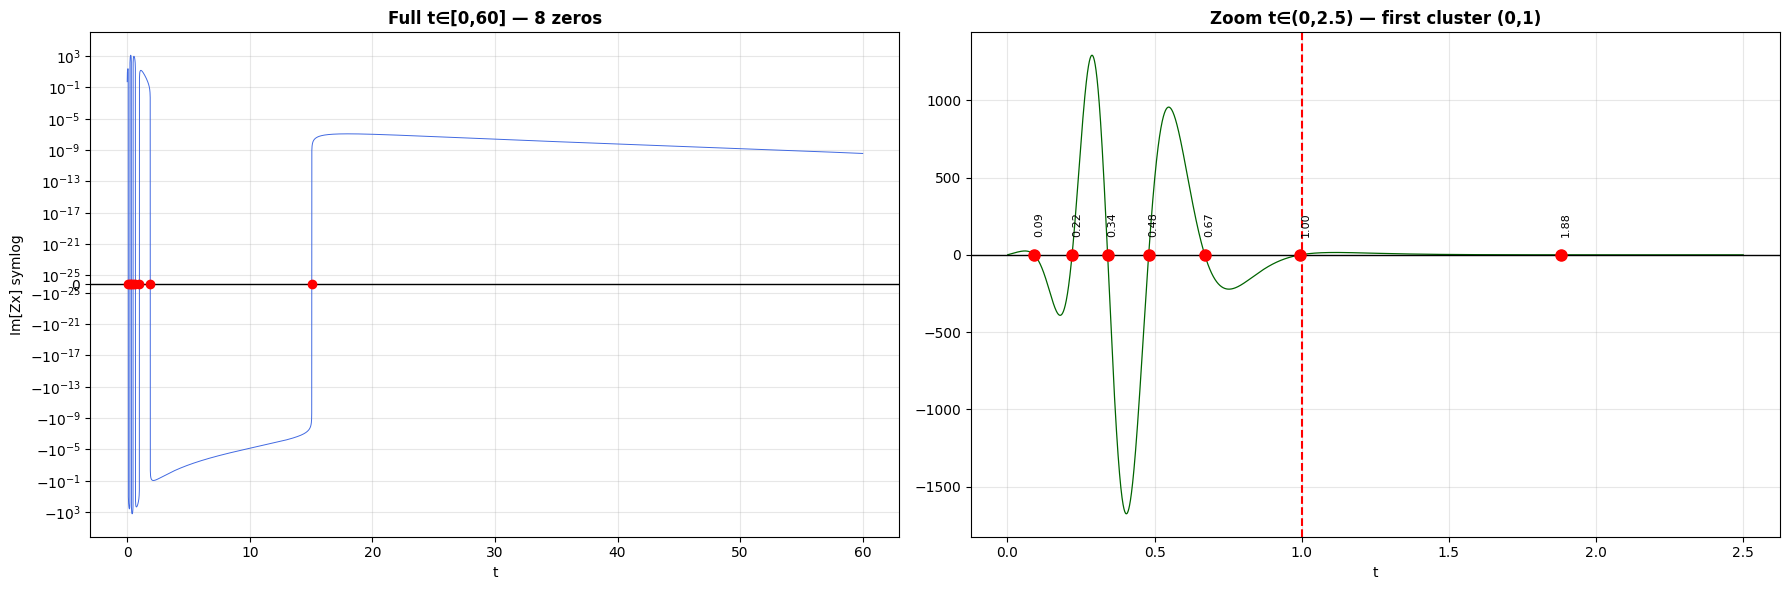
\includegraphics[width=0.95\textwidth]{jabri_5.png}
\caption{Imaginary part of $Z(\tfrac12+it)$ on the critical line.
Left: full range $t\in[0,60]$ on a symlog scale.
Right: zoom over $t\in(0,2.5)$ showing the six zeros in the unit
interval. Red dots mark the eight zeros listed in Table~\ref{tab:zeros}.}
\label{fig:zeros}
\end{figure}

For $t>15.06$, the modulus $|\Im[Z(\tfrac12+it)]|$ remains below
$10^{-6}$ and no further sign change is detected.

\section{Summary}

The field $Z(x)=x^{-5}\ln(x)\sin(2\pi/x)e^{-x/21}$ possesses an
explicit zero set $w_n = 2/n$ on the positive real axis
(Proposition~\ref{prop:real-zeros}) and exhibits exactly eight
numerical zeros on the Riemann critical line for $t\in[0,60]$.
The construction is elementary, the code is short, and the result
is reproducible at 80-digit precision.

\vspace{1em}
\noindent\textbf{Code and data:}\\
\url{https://github.com/jabri62018/Jabri-RiemannOS}

\vspace{0.5em}
\noindent\textbf{Keywords:} elementary scalar field, Riemann critical
line, numerical zero search.

\vspace{0.8em}
\noindent\textit{Sana'a, Yemen --- October 2026}\\
\noindent\texttt{jabri62018@gmail.com}

\end{document}